%%%%%%%%%%%%%%%%%%%%%%%%%%%%%%%%%%%%%%%%%%%%%%%%%%%%%%%%%%%%%%%%%%%
%%% Documento LaTeX 																						%%%
%%%%%%%%%%%%%%%%%%%%%%%%%%%%%%%%%%%%%%%%%%%%%%%%%%%%%%%%%%%%%%%%%%%
% Título:		Capítulo 1
% Autor:  	Ignacio Moreno Doblas
% Fecha:  	2014-02-01, actualizado 2019-11-11
% Versión:	0.5.0
%%%%%%%%%%%%%%%%%%%%%%%%%%%%%%%%%%%%%%%%%%%%%%%%%%%%%%%%%%%%%%%%%%%
% !TEX root = A0.MiTFG.tex
\chapterbegin{Manual básico de \LaTeX}
\label{chp:ManLaTeX}
\minitoc

\begin{sinopsis}
\label{sec:chpltx:sinop}
Éste es el primer capítulo de desarrollo del proyecto, definido y estructurado según el autor necesite y desee. En este caso, no hay guías genéricas para cualquier proyecto más allá del manual de estilo disponible en~\cite{GuiaEstilo}~\footnote{\url{https://www.uma.es/media/tinyimages/file/Manual_de_estilo_ETSIT_TFG_TFM_PFC.pdf}}.

En esta plantilla, este capítulo se enfoca como un manual básico de \LaTeX\ para cualquiera que lo necesite. Como plantilla, está basada en la \ttw{\textbackslash documentclass} tipo \ttw{book}, empleando partes, capítulos, secciones, etc. \LaTeX\ es una herramienta muy orientada a documentos que contienen tablas, figuras, referencias cruzadas, bibliografía, glosarios, apéndices, ecuaciones matemáticas o unidades físicas.
\end{sinopsis}

\section{Estructura y formato del proyecto}
\label{sec:EstrForm}
Esta plantilla sigue las especificaciones de la ETSIT para presentar un TFG/TFM. Igualmente, la plantilla con su material adicional está disponible en la \tit{web} del centro (\url{www.etsit.uma.es}.)

\section{Apartados de la plantilla}

La plantilla está estructurada en los siguientes archivos y directorios:

\begin{itemize}
	\item{Veintitrés ficheros \TeX\ (extensión \ttw{.tex}).}

	\item{Un fichero Bib\TeX\ (extensión \ttw{.bib}).}

	\item{Un fichero PDF resultante.}

	\item{Dos ficheros \TeX nicCenter (extensión \ttw{.tps} y \ttw{.tcp}) por si quieres utilizar este entorno (aunque ha quedado un poco anticuado).}

	\item{Dos directorios complementarios.
		Uno de código fuente (\ttw{code}) y otro de gráficos (\ttw{figuras}).}

\end{itemize}

Existen varias alternativas para trabajar con documentos \LaTeX, como \TeX maker, \TeX studio, o con cualquier editor de texto y el entorno de compilación de \LaTeX\ (MiKTeX --Windows--, LiveTeX --Linux--, MacTeX, --MacOS--). Otra alternativa muy popular es  Overleaf (\url{www.overleaf.com}) que permite la edición on-line y colaborativa con otros usuarios.

\begin{figure}[ht]
	\centering
		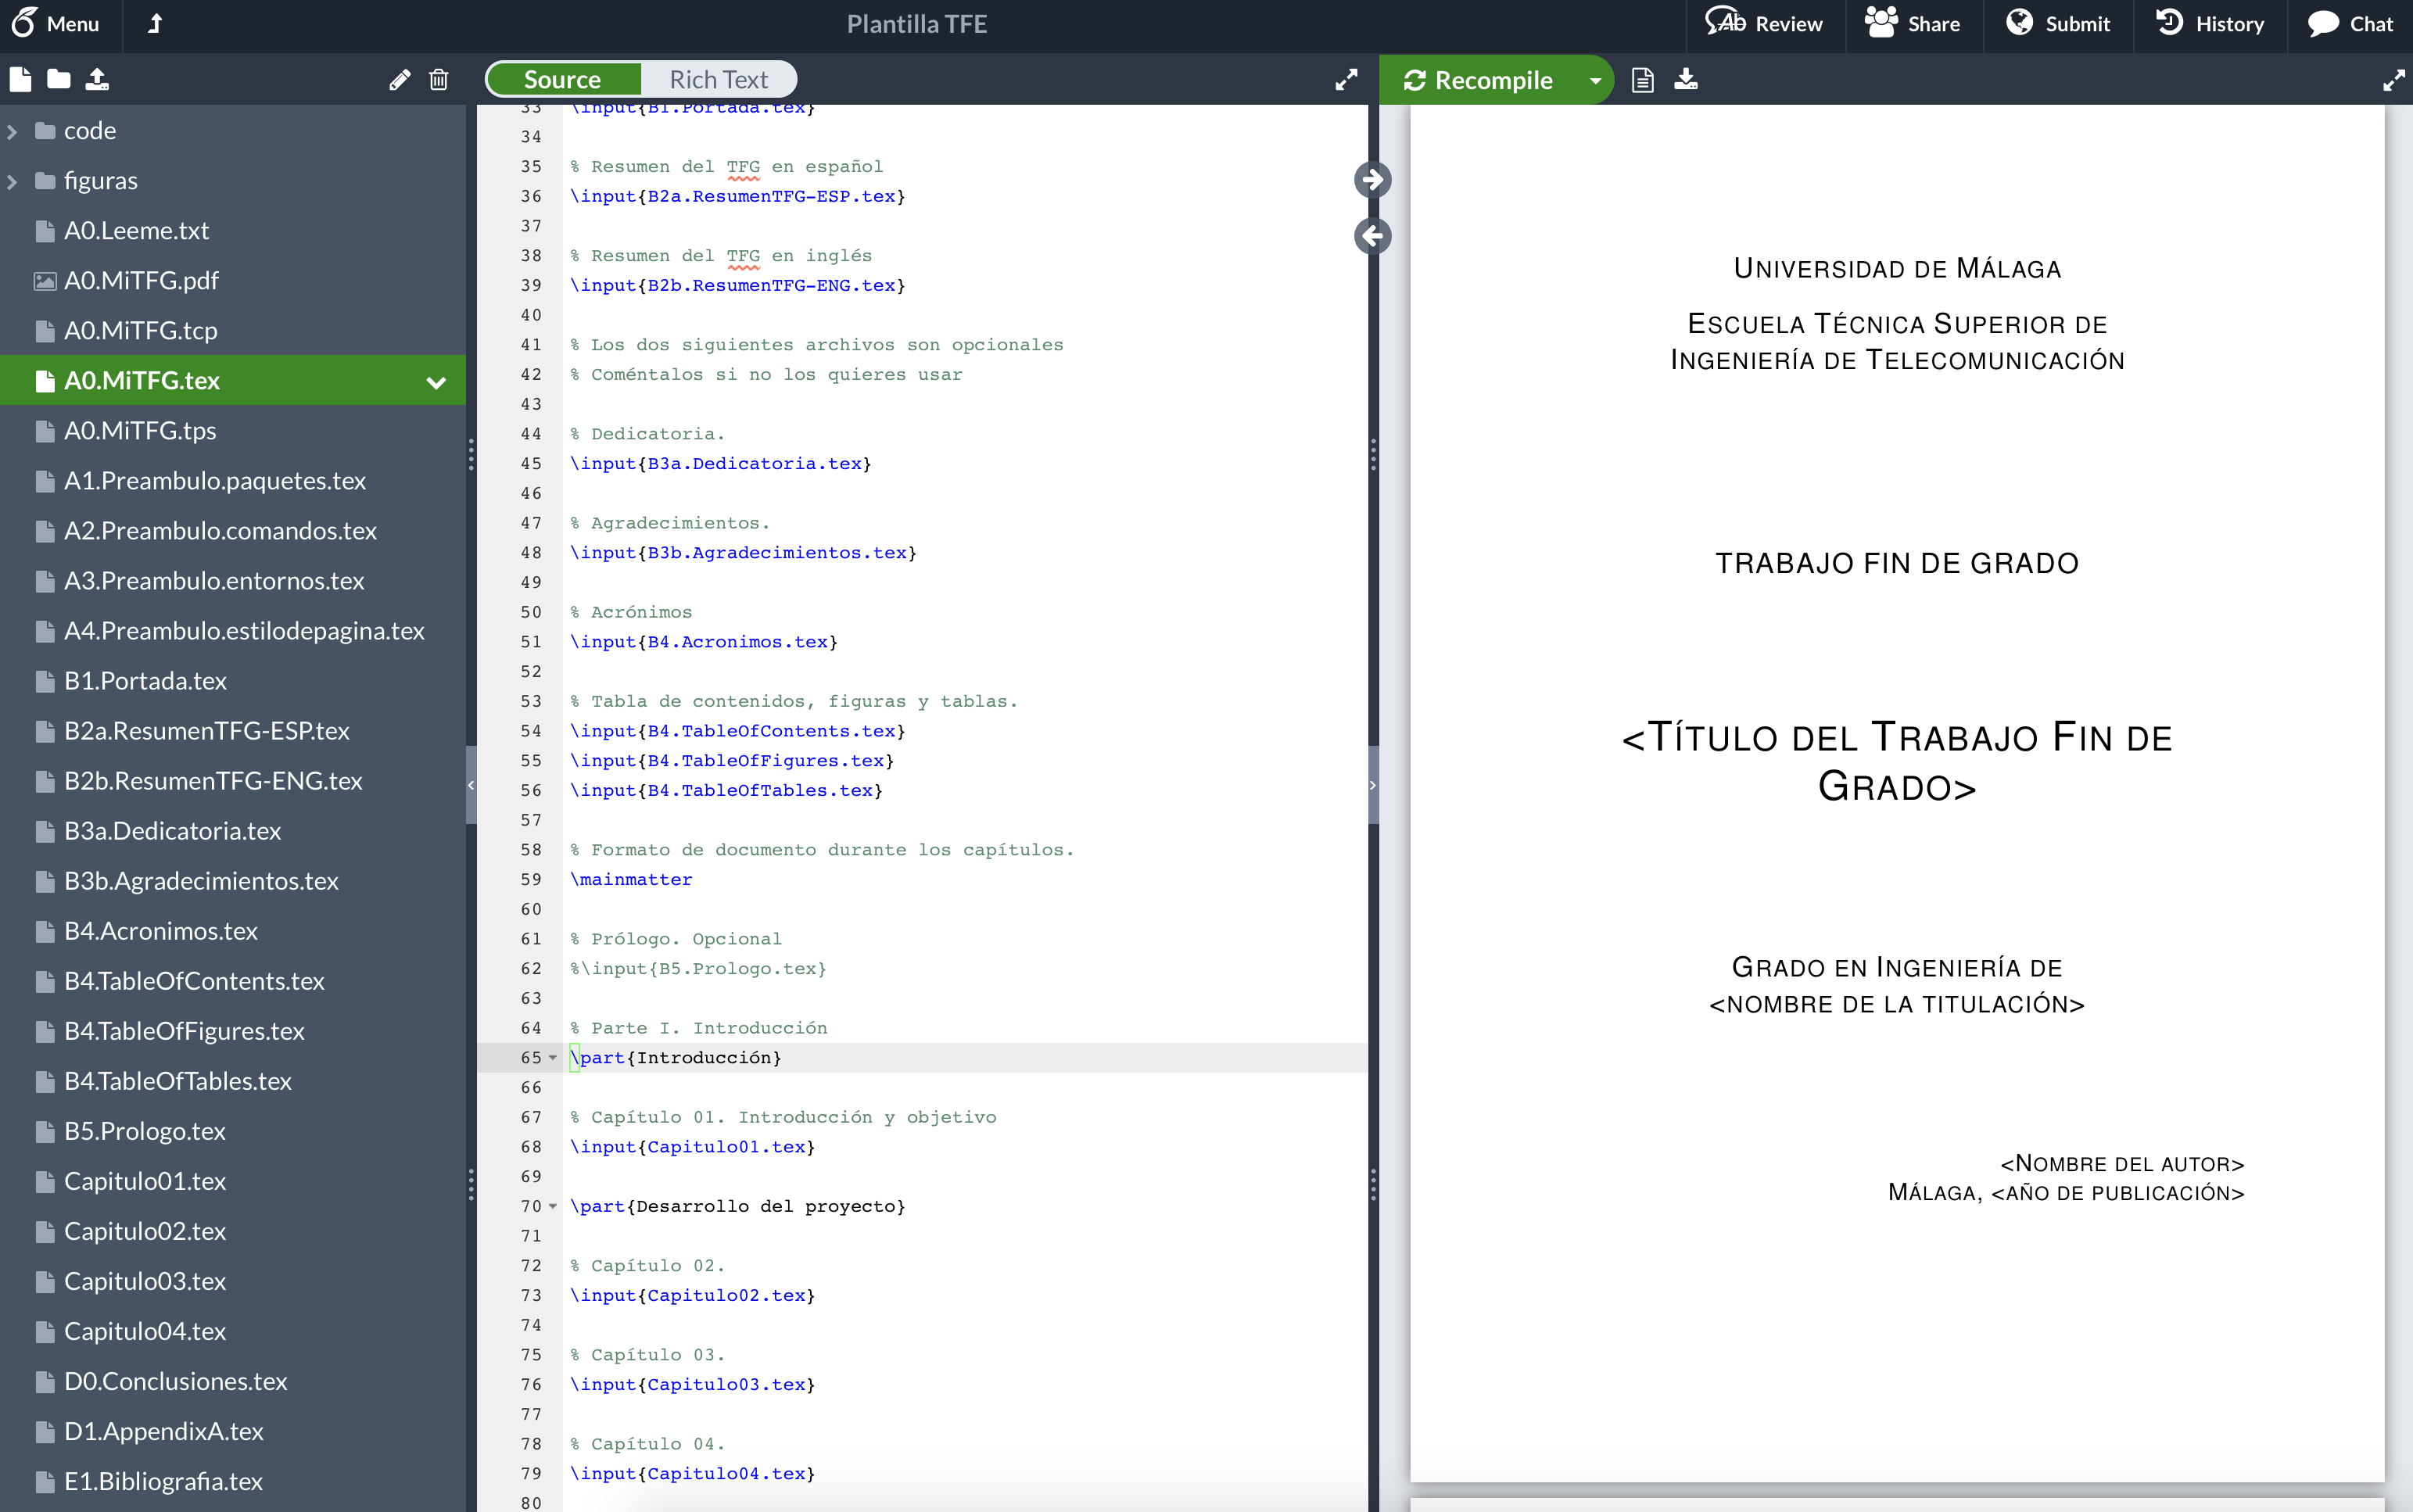
\includegraphics[width=\linewidth]{figuras/overleaf.png}
	\caption{Ficheros de la plantilla y aspecto de Overleaf}
	\label{fig:ficherosPlan}
\end{figure}

En la figura~\ref{fig:ficherosPlan}, puede verse la lista de ficheros del proyecto, tal y como se presenta en el entorno Overleaf. A su vez, entre los veintitrés ficheros \TeX\ encontramos un documento maestro (\ttw{A0.MiTFG.tex}) a partir del cual se referencia el resto de archivos, los cuales se reparten en cuatro clases.

Los archivos contienen un prefijo que hace que su posición en la lista sea equivalente al orden en el documento PDF resultante. Este prefijo es una letra y un número en arábigo. Por ejemplo, el documento maestro, ``\ttw{A0.MiTFG.tex}'', comienza por \ttw{A0} para que figure en primer lugar.

Las cuatro clases de archivos antes mencionadas son las siguientes:

\begin{descript}
	\item[Archivos de preámbulo] Forman el preámbulo del documento \LaTeX\ y su contenido no se visualiza en el fichero PDF resultante. Comienzan por la letra \ttw{A}
	\item[Archivos iniciales] Son los archivos iniciales del proyecto, desde la portada, dedicatoria, acrónimos, tablas de contenido y prólogo. Comienzan por la letra \ttw{B}.
	\item[Archivos de capítulo] Son los ficheros de capítulo del proyecto. Dado que su primera letra coincide con la letra C, no tienen ninguna identificación especial.
	\item[Archivos finales] Por último, los archivos de conclusiones, apéndices, bibliografía y glosario (\tit{index} en inglés).
\end{descript}

En la figura~\ref{fig:ficherosPlan}, segmentada en tres paneles, se observa en la parte izquierda todos estos archivos ordenados según el orden secuencial. Esta ordenación permite una elaboración cómoda del proyecto por lo que se recomienda mantener esta organización. En el panel central se muestra parte del contenido del fichero \LaTeX\ principal y en el panel derecho el fichero PDF al que da lugar después de la compilación.

En el documento PDF resultante, el proyecto se estructura en los nueve apartados siguientes:
\begin{descript}
	\item[Portada y encuadernación.] Es específica de cada tipo de trabajo (TFG/TFM) y debe ajustarse a lo establecido en la Secretaría.

	\item[Primeras páginas.] Contendrá las páginas que correspondan con el tipo de trabajo y que son específicas de cada tipo de proyecto. En el TFG/TFM de la ETSIT estas primeras páginas contienen el título, autor, tutor, resumen y otra identificación del trabajo, tanto en español como en inglés.

	\item[Dedicatoria y agradecimientos.] La sección de agradecimientos (evidentemente, no obligatoria) define un apartado donde el estudiante puede (y quizás, debe) referenciar a aquellas personas y/o instituciones que, de manera generosa, han colaborado de algún modo en la gestación y desarrollo del PFC. Igualmente el estudiante también puede utilizar este apartado libremente para mencionar a aquellos familiares, compañeros, amigos, etc., de los que ha recibido apoyo personal, moral o afectivo. Por contra, no debe utilizarse esta sección para expresar opiniones críticas, ácidas o mordaces contra particulares o instituciones de la ETSIT o la Universidad debido a correcciones, exámenes, trato recibido u otras interacciones o causas cualesquiera que sean, ya que esto estaría fuera del ámbito del proyecto.


	\item[Índice.] En la plantilla, se genera un índice, índice de figuras e índice de tablas, numerado automáticamente con su correspondiente página. Ésta es una de las ventajas de \LaTeX.

	\item[Capítulo 1. Introducción.] En éste se hará una introducción al ámbito del trabajo, comenzando por el contexto general y aproximándose progresivamente a los aspectos más concretos que se traten.	Es conveniente terminar con una exposición clara de los objetivos que se persiguen, la metodología empleada y el contenido del proyecto.

	\item[Capítulos de desarrollo.] A continuación el desarrollo de los distintos capítulos o epígrafes que componen el trabajo. En esta plantilla, éste es el primero de esos capítulos, que además incluye un manual de \LaTeX\ práctico.

	\item[Conclusiones.] En este apartado el estudiante expondrá con claridad los resultados o conclusiones obtenidas y el juicio crítico que le merecen.

	\item[Referencias bibliográficas.] A continuación de las conclusiones se insertará un apartado con todas las referencias bibliográficas que aparezcan en la memoria: revistas, artículos de revistas o congresos, páginas web, etc. En \LaTeX, existe el entorno Bib\TeX\ para almacenar y referenciar bibliografía.

	\item[Apéndices.] Finalmente se presentarán los apéndices, si los hubiere. En esta plantilla se provee del entorno \ttw{\textbackslash appendix} para crearlos.
\end{descript}

Por último, respecto de las secciones del proyecto, hay que tener en cuenta que un proyecto puede ser un documento extenso, complejo y por eso se recomienda seguir este tipo de reglas para facilitar su elaboración. Además, se recomienda generarlo incrementalmente, anulando las secciones que no se utilicen desde el documento maestro. Por ejemplo, al elaborar el capítulo tres y generar el documento PDF, no es necesario ni el prólogo, ni los capítulos anteriores ni posteriores, por tanto, pueden comentarse con el símbolo tanto por ciento (\ttw{\%}) en el documento maestro (A0.MiTFG.tex). En ese caso, la compilación será más rápida, el PDF más breve y la revisión también.

\section{Referencias Cruzadas}
\label{sec:RefCruz}

Normalmente, surge la necesidad de referenciar información desde una sección de la documentación hasta otra. Esta información referenciada puede ser un apartado, una figura, una tabla, una página o una ecuación.

Por ejemplo, el presente capítulo~\ref{chp:ManLaTeX} comienza en la página~\pageref{chp:ManLaTeX} y está titulado \nameref{chp:ManLaTeX} (para generar estas tres referencias en el documento se han usado los comandos \LaTeX\  \verb|\ref{chp:ManLaTeX}|, \verb|\pageref{chp:ManLaTeX}| y \verb|\nameref{chp:ManLaTeX}|, respectivamente, ya que el \verb|\chapter| está etiquetado con \verb|\label{chp:ManLaTeX}|). Es decir, tanto el número de capítulo, su página o su título no están escritos manualmente, sino referenciados mediante etiquetas.

Las referencias cruzadas se realizan siguiendo los siguientes pasos:

\begin{enumerate}

	\item Se etiqueta el elemento a referenciar, ya sea sección, apartado, figura, tabla, ecuación o cualquier otro con el comando \verb|\label{}|. Para ello, se escribe próximo a él un identificador con el comando \verb|\label{}|. Por ejemplo, \verb|\label{sec:RefCruz}| es la etiqueta del presente apartado. Se recomienda, en general, usar como prefijo \ttw{chp} para capítulos, \ttw{sec} para secciones, \ttw{eq} para ecuaciones, \ttw{fig} para figuras o \ttw{tab} para tablas. También usar los dos puntos (:) como separador entre el prefijo y el resto de la etiqueta. A lo largo de esta plantilla pueden encontrarse muchas etiquetas de ejemplo.

	\item Se compila si es la primera vez que se crea la etiqueta. Aunque este paso depende del compilador, en el caso de MiK\TeX\ es necesario compilar para indexar la etiqueta y poder referenciarla, como se indica en el paso siguiente.

	\item Se referencia una etiqueta ya definida con el comando \verb|\ref{}|. Por ejemplo, \verb|\ref{sec:RefCruz}| referencia el presente apartado, cuyo valor es \ref{sec:RefCruz}.

	\item Se compila el documento para crear la referencia a partir de los índices generados en la compilación anterior. Esto es especialmente importante, porque la referencia se crea a partir de la compilación anterior. Si el apartado cambia de página, se debe re-compilar para actualizar la referencia; si no se compila, la referencia se hará según la información desactualizada, es decir, a la página anterior. \emph{En general y términos prácticos, se debe compilar frecuentemente para tener siempre información actualizada.}

\end{enumerate}

Muchos de los entornos para compilar \LaTeX\ son capaces de compilar repetidas veces de forma automática hasta que se resuelven las referencias cruzadas. Entre ellos encontramos Overleaf o Atom con el paquete LaTeX, pero también se puede conseguir el mismo efecto compilando desde una consola usando el comando ``\texttt{make}'' o el comando ``\texttt{latexmk -pdf A0.MiTFG.tex}''.

%\section{Formato de otros elementos}
\section{Figuras}

Las figuras aparecerán centradas y se verán siempre acompañadas por un título explicativo, también centrado y situado en la parte inferior. El título comienza por la palabra ``Figura'' con un identificador de figura formado por el número de capítulo y el número de figura. El propio título debe ser lo bastante explicativo para poder entender el significado de la figura o distinguirla de las demás, pero no debe ser demasiado extenso ya que dificultaría la legibilidad. Para cualquier explicación o justificación más extensa, se debe describir en un párrafo aparte, utilizando referencias cruzadas. Además, tanto el título como el identificador aparecerán referenciados en el índice de figuras al principio de la memoria (esto último ya se consigue de forma automática al compilar).


	En \LaTeX, el entorno \ttw{figure} automatiza la presentación de figuras siguiendo estas reglas. A continuación se ve el texto original utilizado para la figura~\ref{fig:marcaETSIT} de la página~\pageref{fig:marcaETSIT}, titulada \nameref{fig:marcaETSIT}.
	Para respetar los espacios y el texto original se ha utilizado el entorno \ttw{lstlisting}.

\lstset{
  language=[LaTeX]TeX, framexleftmargin=0mm, frame=shadowbox,
  rulesepcolor=\color{gray}, numberstyle=\tiny,
  keywordstyle=\color{blue}\bfseries
}

\begin{lstlisting}[numbers=left,morekeywords={includegraphics}]
\begin{figure}[ht]
	\centering
	
\includegraphics[width=3cm]{figuras/MarcaETSIT.pdf}
	\caption{Marca Teleco de la ETSIT en la UMA}
	\label{fig:marcaETSIT}
\end{figure}
\end{lstlisting}

\begin{figure}[ht]
	\centering
		
\includegraphics[width=9cm]{figuras/MarcaETSIT.pdf}
	\caption{Marca Teleco de la ETSIT en la UMA}
	\label{fig:marcaETSIT}
\end{figure}

Puede ser necesario presentar una figura conteniendo varias en su interior. En ese caso, el entorno \verb|\minipage| puede cumplir esta función aunque se recomienda como mejor alternativa el uso del paquete \texttt{subcaption}. En la figura~\ref{fig:marca:UMA}, se muestran los dos marcas de la Universidad de Málaga usando el entorno \verb|\minipage|.

	\begin{figure}[ht]
		\centering
			\begin{minipage}[l]{6cm}
			\includegraphics[width=6cm]{figuras/MarcaUMA.pdf}
			\end{minipage}
			\ \
			\begin{minipage}[r]{6cm}
			
\includegraphics[width=6cm]{figuras/marcaumaes.pdf}
			\end{minipage}
		\caption{Marcas oficiales de la UMA}
		\label{fig:marca:UMA}
	\end{figure}

La alternativa que ofrece el paquete \texttt{subcaption} permite la utilización del entorno \verb|\subfigure| y ofrece mayor funcionalidad como vemos en la Figura~\ref{fig:marcaUMA}. Cada ``subfigura'' puede tener su propio \texttt{caption}, el cual se puede referenciar como Figura~\ref{fig:marcaUMA-a} y Figura~\ref{fig:marcaUMA-b}.

	\begin{figure}[ht]
	  \centering
	  \begin{subfigure}[t]{0.4\linewidth}
	    \centering
	    \includegraphics[width=\textwidth]{figuras/MarcaUMA.pdf}
			\caption{Marca UMA.}
	    \label{fig:marcaUMA-a}
	  \end{subfigure}%
		\hfill
	  \begin{subfigure}[t]{0.4\linewidth}
	    \centering
	    
\includegraphics[width=\textwidth]{figuras/marcaumaes.pdf}
	    \caption{Marca uma.es.}
	    \label{fig:marcaUMA-b}
	  \end{subfigure}
	  \caption{Las dos marcas de la UMA.}
	  \label{fig:marcaUMA}
	\end{figure}

También es importante conocer algunas características sobre los gráficos vectoriales y de tipo bitmap (también llamados rasterizados\footnote{en inglés, \tit{raster}.}) y sobre los formatos aceptados por \LaTeX\ para gráficos. En general, hay dos tipos de ficheros gráficos en un ordenador:

\begin{descript}
	\item[Bitmap o rasterizados] El gráfico está formado por una matriz de píxeles, como en una fotografía digital.
	Ejemplos de formatos bitmap son JPG, PNG, GIF o TIFF.

	\item[Vectoriales] El gráfico está formado por curvas geométricas, lo que hace que independientemente de la escala mostrada, se mantenga la misma definición, tanto en color como en forma.
	Ejemplos de formatos vectoriales son EPS (\tit{Encapsulated PostScript}), PDF o SVG (\tit{Scalable Vector Graphics}).
	Un ejemplo concreto es la figura~\ref{fig:marcaETSIT}, que está en PDF.
\end{descript}

	Si se desea insertar un gráfico vectorial y se emplea el compilador \ttw{pdflatex} o el comando \texttt{latexmk -pdf}, el formato del gráfico debe ser PDF.
	Si los gráficos vectoriales están en otro formato, tales como SVG o EPS, es necesario usar un conversor.
	Una opción sencilla y gratuita es el editor Inkscape\R, disponible en Internet. No es necesario instalarlo, ya que puede encontrarse una edición portable, que sólo requiere ser descomprimida y ejecutada.

\section{Tablas}
	La presentación de las tablas es equivalente a la de las figuras, tanto en su posición centrada como en su título. En \LaTeX\ existen varios entornos para presentar una tabla, dependiendo de qué se desee:

	\begin{ite}
		\item El entorno \tbf{\ttw{tabular}} permite crear una tabla a partir de definir sus filas, columnas y su formato.
		Está limitado a no poder fragmentarse en varias páginas si la tabla es demasiado extensa.

		\item El entorno \tbf{\ttw{table}} formatea una tabla, una sección de código fuente o algún componente equivalente.
		Permite posicionar, ponerle un título y añadirlo al índice de tablas. En el ejemplo siguiente, se utilizan los dos entornos, uno \ttw{table} y otro \ttw{tabular} anidado en el primero.

		\item El entorno \tbf{\ttw{longtable}} es equivalente a \ttw{tabular}, pero además supera la limitación de extender una tabla a más de una página.
	\end{ite}

	De nuevo, las tablas aparecen referenciadas en un índice de tablas tras el índice temático y del índice de figuras.

	A continuación, se muestra el código \LaTeX\ de la tabla~\ref{tab:SAR}, presente en la página~\pageref{tab:SAR}, titulada \nameref{tab:SAR}.

\begin{lstlisting}
\begin{table}[ht]
\centering
\begin{tabular}{|c|p{14ex}|c|c|}
	\hline \hline
	\tbf{Requisito} & \tbf{Plat. Referencia} &
		\tbf{SAR (dBm)} & \tbf{Tol.}\\ \hline
	R101  &  Baytrail 		& 5 & 1 \\ \hline
	R201  &  Clovertrail 	& 6 & 2 \\ \hline
	R301  &  Merrifield 	& 4 & 3 \\ \hline \hline
\end{tabular}
\caption{Tabla de SAR por Plat. de Referencia}
\label{tab:SAR}
\end{table}
\end{lstlisting}

	%\begin{center}
	\begin{table}[ht]%
	\centering
	%\begin{longtable}{c|p{10cm}}
	\begin{tabular}{|c|p{14ex}|c|c|}
		\hline \hline
		\tbf{Requisito} & \tbf{Plat. Referencia} &
			\tbf{SAR (dBm)} & \tbf{Tol.}\\ \hline
		R101  &  Baytrail 		& 5 & 1 \\ \hline
		R201  &  Clovertrail 	& 6 & 2 \\ \hline
		R301  &  Merrifield 	& 4 & 3 \\ \hline \hline
	\end{tabular}
	\caption{Tabla de SAR por Plat. de Referencia}
	\label{tab:SAR}
	\end{table}
	%\end{longtable}
	%\end{center}%\end{table}

\section{Código fuente}

En un proyecto de desarrollo, es común introducir extractos de código en diferentes lenguajes como C, C++, Matlab, Python, Java, bash script, etc. En estos casos, los entornos de \LaTeX\ disponibles por defecto no permiten mostrar esta información.

El paquete \ttw{listings} es muy utilizado para presentar código fuente, respetando las tabulaciones para que la lectura sea confortable. En esta plantilla, en la sección de paquetes (fichero \texttt{A1.Preambulo.paquetes.tex}) se ha configurado el paquete \texttt{listings} para que use el lenguaje Python a la hora de presentar código con resaltado de sintaxis (\emph{syntax highlighting}). 

Este paquete es fácilmente adaptable para otros lenguajes y de hecho, en los listados \LaTeX\ con los ejemplos de uso del entorno \texttt{figure} y \texttt{table} mostrados previamente, se ha configurado \texttt{listings} para que resalte la sintaxis de código \LaTeX.

En la sección de comandos, se ha definido el comando \ttw{code}, el cual permite crear una sección de código siempre que indiquemos los tres argumentos entre llaves:
\begin{itemize}
    \item título a mostrar
    \item fichero fuente correspondiente
    \item etiqueta con la que se harán referencias a dicho Listado
\end{itemize}

Por ejemplo, mediante el comando: 

\begin{verbatim}
	\code{Ejemplo de código Python}{code/pythonCode.py}{code:python}
\end{verbatim}

\noindent conseguimos el Listado~\ref{code:python}.

\lstset{
  language=Python, %Puede ser C, C++, Java, etc.
  showstringspaces=false,
  formfeed=\newpage,
  tabsize=4,
  commentstyle=\itshape,
  morekeywords={models, lambda, forms}
}

\code{Ejemplo de código Python}{code/pythonCode.py}{code:python}

El paquete \texttt{listings} es muy completo y configurable\footnote{Ver \url{http://texdoc.net/texmf-dist/doc/latex/listings/listings.pdf} si quieres ver todas las opciones y sacarle el máximo jugo.}. Por ejemplo, con el siguiente código \LaTeX:

\begin{verbatim}
\begin{minipage}{0.96\linewidth}
  \begin{center}
    \begin{lstlisting}[language={[11]C++}, frame=lines, numbers=left,
        numberstyle= \tiny,	keywordstyle=\color{blue}\bfseries,
        framexleftmargin = 5mm,
        caption={Hola mundo en C++},
        label={code:holaC++}]
#include <iostream>
int main(){
  std::cout << "Hola mundo\n";(@\label{lst:cout}@)
  return 0;
}
    \end{lstlisting}
  \end{center}
\end{minipage}
\end{verbatim}

\noindent obtenemos el Listado \ref{code:holaC++}, donde hemos insertado una \texttt{label} que se procesa en \LaTeX\ gracias a los comandos de escape \texttt{(@} y \texttt{@)}, y por tanto podemos hacer referencia a la línea del Listado que queramos explicar. Por ejemplo, la línea~\ref{lst:cout} del Listado~\ref{code:holaC++} provoca que se imprima la cadena ``Hola mundo'' cuando se ejecuta el programa.

\begin{minipage}{0.96\linewidth}
\begin{center}
    \begin{lstlisting}[
        language   = {[11]C++},
        frame      = lines,
	    numbers		 = left,
		numberstyle= \tiny,
		keywordstyle=\color{blue}\bfseries,
		framexleftmargin = 5mm,
        caption    = {Hola mundo en C++},
        label      = {code:holaC++}
    ]
#include <iostream>
int main(){
  std::cout << "Hola mundo\n";(@\label{lst:cout}@)
  return 0;
}
\end{lstlisting}
\end{center}
\end{minipage}

\section{Símbolos matemáticos y físicos}
Los proyectos de ingeniería suelen presentar símbolos matemáticos y físicos, tanto en los párrafos como en tablas, figuras y ecuaciones. Existen reglas para la notación, formateo y estilo de elementos matemáticos, tales como utilizar un símbolo por variable (p.ej., $x$ e $y$, pero no $xx$ o $yy$), escribir los símbolos en cursiva y las magnitudes y unidades físicas en redonda o el espaciado entre variables.

\LaTeX\ está construido sobre \TeX, que fue concebido originalmente para escribir textos matemáticos con alta calidad, de forma que funciona perfectamente en estos entornos. Su integración es suave, rápida y sencilla de seguir, una vez se tiene algo de práctica.
Esta facilidad se hace extensiva al uso de magnitudes físicas con sus correspondientes múltiplos. \LaTeX\ ofrece el paquete \ttw{SIunits}, ya incluído en esta plantilla.

A continuación se muestran varios ejemplos de su uso, con su código original. Para ecuaciones integradas en el párrafo, tan sólo se usa el símbolo dólar (\$) antes y después del símbolo. Por ejemplo, con \verb|$x$| se indica la variable $x$. Las ecuaciones en línea deben usarse para expresiones cortas y que no requieran de mucho espacio vertical. Para escribir ecuaciones más largas están los entornos \ttw{displaymath}, \ttw{equation} y \ttw{align}.

Los entornos \ttw{displaymath} y \ttw{equation} muestran una ecuación en una línea. La diferencia entre ambos es que el primero no realiza una numeración de la ecuación y el segundo sí. Sólo se pueden referenciar las ecuaciones numeradas.

Por ejemplo, la ecuación de la proporción áurea en entorno \ttw{displaymath},

\lstset{language=[LaTeX]TeX,
keywordstyle=\color{blue}\bfseries
}
\begin{lstlisting}
	\begin{displaymath}
		\phi^2 - \phi - 1 = 0
	\end{displaymath}
\end{lstlisting}

\begin{displaymath}
	\phi^2 - \phi - 1 = 0
\end{displaymath}

\noindent mientras que si usamos el entorno \ttw{equation}, mostraremos la ecuación~\ref{eq:aurea} en la página~\pageref{eq:aurea}:
\begin{lstlisting}
	\begin{equation}
		\phi^2 - \phi - 1 = 0
		\label{eq:aurea}
	\end{equation}
\end{lstlisting}

\begin{equation}
	\phi^2 - \phi - 1 = 0
	\label{eq:aurea}
\end{equation}

%\begin{equation}
	%\int_0^\infty \mathrm{e}^{-x}\,\mathrm{d}x = z
	%\label{eq:prueba}
%\end{equation}

En caso de querer desarrollar una ecuación en varias líneas, se debe emplear el entorno \ttw{align}. Funciona como un entorno \ttw{array} de dos columnas separadas por el símbolo dólar. Por ejemplo, el desarrollo en serie de Fourier de una función $x(t)$ en forma trigonométrica y exponencial,
\begin{align}
	x(t) & = \frac{a_0}{2} %\\
	     + \sum_{k = 1}^{k = \infty}{A_k \cos(\omega_{k} t)}
			 + \sum_{k = 1}^{k = \infty}{B_k \sin(\omega_{k} t)}\label{eq:fou:trig} \\
			 & = \sum_{k = -\infty}^{k = \infty}{X_k e^{j \omega_k t}}\label{eq:fou:exp}
\end{align}

Referenciando ambas ecuaciones, la ecuación~\ref{eq:fou:trig} desarrolla la serie de Fourier de forma trigonométrica y la ecuación~\ref{eq:fou:exp} de forma exponencial.

En caso de no querer mostrar ninguna numeración en las ecuaciones, se debe usar el entorno \ttw{align*}. En caso de querer desarrollar una ecuación, pero sólo numerar algunas de ellas, se debe añadir el comando \ttw{\textbackslash nonumber} a las ecuaciones que no deseen ser numeradas. Como anotación, existe también el entorno \ttw{eqnarray}, pero presenta limitaciones, tales como referenciar varias ecuaciones dentro de un entorno. Por esta razón es mejor usar el entorno \ttw{align}.

Respecto a las magnitudes y unidades físicas, la tabla~\ref{tab:ctes} (pág.~\pageref{tab:ctes}) muestra diferentes constantes físicas.

\begin{table}[h]
\centering
\begin{tabular}{p{8cm}cp{3cm}}
	\hline
	Constante Gravitacional & $G_0$ & $6.67 \, 10^{-11} \, \newton\metre^2\per\kilogram^2$\\
	Constante de Planck & $h$ & $6.63 \, 10^{-34} \, \joule\cdot\second$\\
	Constante de Stefan-Boltzman & $\sigma$ & $5.67 \, 10^{-8} \watt\per\metre^2\kelvin^4$\\
	Carga elemental & $e$ & $1.6 \cdot 10^{-19} \, \coulomb$\\
	Masa del electrón & $m_e$ & $9.11 \, 10^{-31} \kilogram$\\
	Velocidad de la luz en el vacío & $c_0$ & $3 \, 10^8 \metre\per\second$ \\
	Permitividad eléctrica en el vacío & $\epsilon_0$ & $8.85 \, 10^{-12} \, \farad\per\metre$\\
	Permeabilidad magnética en el vacío & $\mu$ & $1.26 \, 10^{-6} \, \henry\per\metre$\\
	\hline
\end{tabular}
	\caption{Constantes físicas (usando \ttw{SIunits})}
	\label{tab:ctes}
\end{table}

En el manual de \ttw{SIunits}, presente en un PDF entre el material adicional adjunto a esta plantilla, se puede encontrar el resto de magnitudes y unidades a utilizar (especialmente, pág.~25 y sigs.).

\section{Referencias bibliográficas}

Además del etiquetado de secciones, tablas, figuras y ecuaciones a lo largo del proyecto, debe referenciarse el origen bibliográfico de todos los datos necesarios.

Para ello, \LaTeX\ incluye la herramienta Bib\TeX, que permite almacenar fuentes bibliográficas (libros, artículos, revistas, páginas web, seminarios, etc.) en un archivo y formato estándar, referenciarlas mediante etiquetas (equivalente a las referencias a secciones, tablas, figuras y ecuaciones) y variar el estilo bibliográfico según se prefiera. En esta plantilla se incluyen dos ficheros,
\begin{ite}
	\item \ttw{E2.Bibliografia.bib}. Fichero que contiene todas las fuentes bibliográficas utilizando la estructura de Bib\TeX.
	\item \ttw{E1.Bibliografia.tex}. Fichero que al final de la memoria  imprime las referencias según el estilo bibliográfico seleccionado entre varias opciones. También incluye la referencia a la bibliografía en la Tabla de contenidos del proyecto.
\end{ite}

Respecto al estilo bibliográfico, el autor puede seleccionar el que considere mejor según su criterio. Bib\TeX\ ofrece los siguientes estilos bibliográficos:
\begin{descript}
	\item[plain] Es el estilo básico (de ahí, su nombre). Las entradas se ordenan alfabéticamente y se etiquetan con un número (p.ej., [1]).
	\item[unsrt] Es igual que plain, pero aparecen en orden de citación.
	\item[alpha] El etiquetado se hace por autor y año de publicación (p.ej., [Knu66])
	\item[abbrv] Igual que alpha, pero más abreviado.
\end{descript}

	Comparando esta plantilla con la guía de estilo (véase~\cite{GuiaEstilo}, pág. 13 y sigs.), los estilos \ttw{plain} y \ttw{unsrt} corresponden con el denominado método numérico y los estilos \ttw{alpha} y \ttw{abbrv} con el método autor y año.

\section{Formato de los Apéndices}
	Se incluye en los apéndices información complementaria al texto del proyecto que no se considera indispensable para su compresión.

	Ejemplo: Apéndice A: Métodos de generación de ruidos gaussianos fraccionarios.

	Los apéndices se numeran alfabéticamente y para su redacción, se han de seguir las reglas de seccionado como en los capítulos anteriores.

\section{Glosario de términos}
Un glosario (en inglés, \tit{index}) referencia palabras importantes dentro del documento y la página o páginas en que puede encontrarse este término. En \LaTeX, la herramienta \ttw{MakeIndex} presente en el paquete \ttw{makeidx} se encarga de gestionar los apéndices. Esta plantilla ya incluye este paquete.

Aunque \ttw{MakeIndex} ofrece muchas más prestaciones, se muestra un uso básico con el comando \ttw{\textbackslash miindex}. Con él se crea la palabra seleccionada y se inserta en el glosario con su correspondiente referencia a la página en la que aparece el término. Por ejemplo, escribiendo \verb|\miindex{glosario}| conseguimos que la plabra \miindex{glosario} aparezca en el glosario de términos al final del documento y referencie la página actual.

\section{Sobre los correctores ortográficos}

\LaTeX\ no incluye un corrector ortográfico como Microsoft Word\R.
Tampoco el compilador \LaTeX, que sólo recibe un fichero fuente en formato TXT y lo entrega en PDF.

Si se desea esta funcionalidad\footnote{Es muy recomendable, en mi opinión (Nota del autor).}, se depende del entorno de desarrollo. Para la mayoría de los editores es posible configurar el corrector ortográfico (\emph{spell checker}) para el idioma en que se esté escribiendo el documento. En Overleaf, el idioma por defecto es el inglés, pero en el ``Menú'' también se puede cambiar a español en el desplegable \emph{spell check}.

\section{Decálogo del usuario novel de \LaTeX}

Como se ha comentado anteriormente, la curva de aprendizaje de \LaTeX\ requiere una pequeña inversión pero se amortizará rápidamente si se van a editar documentos profesionales y de calidad en el futuro (una tesis, un artículo de congreso o revista, un documento técnico, etc.)\footnote{Además hay que añadir que conseguir un documento de equivalente calidad no resulta mucho más fácil en otro sistema, ya que requiere conocer funciones avanzadas.}. Para introducirse progresivamente en la edición en \LaTeX se recomienda seguir estos consejos:

\begin{enumerate}

	\item Sé práctico, aprende lo que necesites para el proyecto de esta plantilla y utilízalo.

	\item Sigue la plantilla, está pensada para proveerte de casi todo lo necesario.

	\item Usa formularios (en inglés, \tit{cheat sheet}) y busca en internet lo que necesites.

	\item Cuanto antes, instálate un entorno \LaTeX\ (MiKTeX -Windows-, LiveTeX -Linux-, MacTeX, -MacOS-) y practica con él.

	\item Practica con el entorno.

	\item Sé paciente, deja que \LaTeX\ te resulte familiar.

	\item Si después de intentarlo, no lo consigues, no lo uses, no es obligatorio.

	\item No te conviertas en tipógrafo, no profundices demasiado.

	\item Concéntrate en el contenido. Deja el estilo para el final.

	\item Cualquier error de compilación \LaTeX\ ya le ha ocurrido a alguien y la solución suele estar a tu alcance buscando la cadena de error en Google o en Stack Overflow.

\end{enumerate}


\section{Otras recomendaciones}

Finalmente, hay cuatro recomendaciones a tener en cuenta durante la redacción del proyecto. Son consejos prácticos basados en la experiencia que resultarán útiles.

\begin{descript}

	\item[Ficheros de compilación.] El compilador de \LaTeX\ genera ficheros de salida tales como el resultado de la compilación (los \tit{logs}), muy importantes en caso de tener que encontrar causas de origen en un fallo; tablas de contenido, tablas de figuras, ficheros que realimentan la siguiente compilación como las referencias cruzadas, o la bibliografía. Como recomendación, mantener estos ficheros actualizados y utilizar las opciones del entorno de desarrollo para borrarlos o guardarlos en una ubicación específica.

	\item[Codificación de archivos] Existen varios formatos de codificación de archivos, que condicionan cómo los ceros y unos representan los caracteres (ANSI, Latin-1, UTF-8, etc.). Dependiendo del formato, el compilador puede malinterpretar los caracteres, generando un documento erróneo, típicamente con los acentos. A veces, incluso, el lector puede leer bien el texto pero el compilador no, siendo más difícil detectar este hecho. La causa es que el editor de texto tiene reglas diferentes del compilador \LaTeX. También es común que ocurra esto en un situación de copiar y pegar texto. En ese caso, debe cambiarse la codificación para que sea correcta. Una forma sencilla de hacerlo en Windows\R\ es utilizando el Notepad++. Hay una opción de codificación. En Linux y Mac dispones del comando \texttt{iconv}.

	\item[Referenciar a ficheros] Para la referencia a ficheros en figuras o a código fuente, hay que usar ficheros. Es recomendable que su nombre tenga un juego de caracteres reducido, es decir, alfanumérico y poco más, y que su ruta de acceso siga esa regla también, es decir, en los directorios relativos respecto del directorio principal. Por ejemplo, en esta plantilla, las gráficas están en el directorio `code' y los gráficos en el directorio `figuras'.

\end{descript}

\chapterend{}
